\documentclass[12pt,]{article}
\usepackage[T1]{fontenc}
\usepackage{lmodern}
\usepackage{amssymb,amsmath}
\usepackage{ifxetex,ifluatex}
\usepackage{fixltx2e} % provides \textsubscript
% use upquote if available, for straight quotes in verbatim environments
\IfFileExists{upquote.sty}{\usepackage{upquote}}{}
\ifnum 0\ifxetex 1\fi\ifluatex 1\fi=0 % if pdftex
  \usepackage[utf8]{inputenc}
\else % if luatex or xelatex
  \ifxetex
    \usepackage{mathspec}
    \usepackage{xltxtra,xunicode}
  \else
    \usepackage{fontspec}
  \fi
  \defaultfontfeatures{Mapping=tex-text,Scale=MatchLowercase}
  \newcommand{\euro}{€}
\fi
% use microtype if available
\IfFileExists{microtype.sty}{\usepackage{microtype}}{}
\usepackage[margin=1in]{geometry}
\usepackage{graphicx}
% Redefine \includegraphics so that, unless explicit options are
% given, the image width will not exceed the width of the page.
% Images get their normal width if they fit onto the page, but
% are scaled down if they would overflow the margins.
\makeatletter
\def\ScaleIfNeeded{%
  \ifdim\Gin@nat@width>\linewidth
    \linewidth
  \else
    \Gin@nat@width
  \fi
}
\makeatother
\let\Oldincludegraphics\includegraphics
{%
 \catcode`\@=11\relax%
 \gdef\includegraphics{\@ifnextchar[{\Oldincludegraphics}{\Oldincludegraphics[width=\ScaleIfNeeded]}}%
}%
\ifxetex
  \usepackage[setpagesize=false, % page size defined by xetex
              unicode=false, % unicode breaks when used with xetex
              xetex]{hyperref}
\else
  \usepackage[unicode=true]{hyperref}
\fi
\hypersetup{breaklinks=true,
            bookmarks=true,
            pdfauthor={},
            pdftitle={},
            colorlinks=true,
            citecolor=blue,
            urlcolor=blue,
            linkcolor=magenta,
            pdfborder={0 0 0}}
\urlstyle{same}  % don't use monospace font for urls
\setlength{\parindent}{0pt}
\setlength{\parskip}{6pt plus 2pt minus 1pt}
\setlength{\emergencystretch}{3em}  % prevent overfull lines
\setcounter{secnumdepth}{0}

\author{}
\date{}
\usepackage{lineno}
\linenumbers
\usepackage{setspace}
\doublespacing
\usepackage{todonotes}

\begin{document}

\normalsize


\begin{centering}
\textbf{\large{Do we need detailed demographic data to forecast the impacts of climate change on plant populations?}}

\textsc{\small{Andrew T. Tredennick\footnote{E-mail: atredenn@gmail.com} and Peter B. Adler}}

\textit{\small{Department of Wildland Resources and the Ecology Center, 5230 Old Main Hill, Utah State University, Logan, Utah 84322-5230 USA}}

\end{centering}

\subsection{Abstract}\label{abstract}

Forecasting future states of populations has taken on new urgency as the
rate of climate change increases. Traditional plant population models
have limited utility in this regard because they are based on detailed
demographic data from small, localized plots. These models are difficult
to scale up to spatial scales relevant to land managers that require
such forecasts to make decisions. To overcome the data limitations of
traditional population models, some have proposed population models
based on population level, rather than individual level, data that is
much easier to collect over broad spatial scales. Using such models
violates a central assumption of ecology: individuals respond to
weather, not populations to climate. Here, we test whether this
assumption is important when forecasting climate change impacts on four
perennial grass species in a semi-arid Montana grassland. We
parameterized two population models, one based on inidividual-level data
with three vital rates and one on population-level data from the same
dataset (percent cover of quadrats), and compared their accuracy,
precision, and sensitivity to climate. The individual level model was
more accurate and precise than the aggregate level model when predicting
out-of-sample observations. When comparing climate effects from both
models, the population-level model tends to ``miss'' important climate
effects from at least one vital rate for each species. We also find that
increasing the sample size at the population-level would not necessarily
reduce forecast certainty; meaning the only way to reduce uncertainty is
to capture unique climate dependence on individual vital rates. It
appears there is no short cut to forecasting climate change impacts on
plant populations --- detailed demographic data is essential. However,
forecasts from our individual-level model were very uncertain, so we
advocate for a focus on new methods to collect demographic data more
efficiently across environmental gradients in space and time.

\emph{Key words: forecasting, climate change, grassland, integral
projection model, population model}

\subsection{Introduction}\label{introduction}

Perhaps the greatest challenge for ecology in the 21st century is to
forecast the impacts of environmental change (Clark et al. 2001, Petchey
et al. 2015). To do so requires sophisticated modeling approaches that
fully account for uncertainty and variability in the ecological process
and associated parameters (Luo et al. 2011). This requires large amounts
of data collected over large spatio-temporal extents.
State-of-the-science modeling techniques cannot overcome data
limitations. Such is the case for many population models.

Population models are important tools for predicting the impacts of
environmental change on species persistence and abundance. But
reconciling the scales at which population models are parameterized and
the scales at which environmental changes play out remains a challenge
(Clark et al. 2010, 2012, Freckleton et al. 2011, Queenborough et al.
2011). The major hurdle is that most population models are built using
data from a single study site because collecting those data, which
involves tracking the fates of individuals plants, is so difficult. The
resulting models cannot be applied to the landscape and regional scales
relevant to decision-makers without information about how the fitted
parameters respond to spatial variation in biotic and abiotic drivers
(Sæther et al. 2007). The limited spatial extent of individual-level
demographic datasets constrains our ability to use population models to
address applied questions about the consequences of climate change.

The inability of many population models to address landscape-scale
problems may explain why land managers and conservation planners have
embraced species distribution models (SDMs) (see Guisan and Thuiller
2005 for a review). SDMs typically rely on easy-to-collect
presence/absence data (but see Clark et al. 2014 for new methods) and
remotely-sensed environmental covariates that allow researchers to model
large spatial extents (e.g., Maiorano et al. 2013). Thus, it is
relatively straightforward to parameterize and project SDMs over
landscapes and regions, the scales at which many land-use decisions are
made. However, the limitations of SDMs are well known (Pearson and
Dawson 2003, Elith and Leathwick 2009, Araújo and Peterson 2012).
Ideally, researchers would provide managers with landscape-scale
population models, combing the extent of SDMs with information about
dynamics and species abundances.

Aggregate measures of population status, rather than individual
performance, offer an intriguing alternative for modeling populations
(Clark and Bjørnstad 2004, Freckleton et al. 2011). Population-level
data cannot provide inference about demographic mechanisms, but it might
be sufficient for modeling future population states, especially since it
is feasible to collect across broad spatial extents (e.g., Queenborough
et al. 2011). The choice between individual and population-level data
involves a difficult trade-off: while individual-level data leads to
more mechanistic models, population-level data leads to models that can
be applied over greater spatial and temporal extents. An open question
is how much forecasting skill is lost when we build models based on
population rather than individual-level data.

To date, most empirical population modelers have relied on
individual-level data, with few attempts to exploit population-level
data. An important exception was an effort by Taylor and Hastings (2004)
to model the population growth rate of an invasive species to identify
the best strategies for invasion control. They used a
``density-structured'' model where the state variable is a discrete
density state rather than a continuous density measure. Such models do
not require individual level demographic data and can adequately
describe population dynamics.

Building on Taylor and Hastings (2004), Freckleton et al. (2011) showed
that density-structured models compare well to continuous models in
theory, and Queenborough et al. (2011) demonstrated the application of
such methods in a study on arable weeds. In particular, Queenborough et
al. (2011) provide empirical evidence that density-structured models are
capable of reproducing population dynamics, even if some precision is
lost when compared to fully continuous models. The study by Queenborough
et al. (2011) included data from 500 fields (4 hectares each) in 49
farms, all collected by two people in 6 weeks. This is far more data
from a far greater spatial extent than possible if measuring individual
plant demography (in a world of limited time and money, at least). The
appeal of density-structured approaches is clear. However, none of these
models included environmental covariates.

Addressing climate change questions with models fit to population-level
data is potentially problematic. It is individuals, not populations,
that respond to climate variables (Clark et al. 2012). Ignoring this
fact puts us in uneasy proximity to an ``ecological fallacy'', where
inference about the individual relies on statistical inference on the
group (Piantadosi et al. 1988). Population growth (or decline) is an
epiphenomenon of demographic processes like survival, growth, and
recruitment that occur at the level of individual plants. Climate can
affect each demographic process in unique, potentially opossing, ways
(Dalgleish et al. 2011). These unique climate responses may difficult
resolve in statistical models based on population-level data where
demographic processes are not identifiable. If population-level data
cannot detect important impacts of climate drivers on populations, then
population models built with such data will make poor forecasts.

Here, we ask whether statistical and population models based on
aggregated, population-level data can detect climate signals as wells as
models based on individual-level data. We used a unique demographic
dataset that tracks the fates of individual plants from four species
over 14 years to build two kinds of single-species population models,
traditional models using individual growth, survival, and recruitment
data and alternative models based on basal cover. In both models,
interannual variation is explained, in part, by climate covariates. We
then performed simulations to quantify the sensitivities of species'
cover to small perturbations in average precipitation and temperature.
We found that population models based on detailed demographic data are
more accurate and precise than models based on aggregated data. Our
results suggest the popuation-level model is less accurate and precise
because important demographic climate signals go undetected. For these
species at this location, detailed demographic data appears necessary to
make accurate forecasts. A worrying caveat to our work is that forecasts
from both models were very uncertain when we considered full process and
parameter uncertainty. Even 14 years worth of demographic data may not
be sufficient to make useful forecasts.

\subsection{Materials and Methods}\label{materials-and-methods}

\subsubsection{Study site and data}\label{study-site-and-data}

Our demographic data come from the Fort Keogh Livestock and Range
Research Laboratory in eastern Montana's northern mixed prairie near
Miles City, Montana, USA ($46^{\circ}$ 19' N, $105^{\circ}$ 48' W). The
dataset is freely available on Ecological Archives\footnote{\url{http://esapubs.org/archive/ecol/E092/143/}}
(Anderson et al. 2011) , and interested readers should refer to the
metadata for a complete description. The site is about 800 m above sea
level and mean annual precipitation (1878-2009) is 334 mm, with most
annual precipitation falling from April through September. The community
is grass-dominated and we focused on the four most abundant grass
species: \emph{Bouteloua gracilis} (BOGR), \emph{Hesperostipa comata}
(HECO), \emph{Pascopyrum smithii} (PASM), and \emph{Poa secunda} (POSE)
(Fig. 1).

From 1932 to 1945 individual plants were identified and mapped annually
in 44 1-$\text{m}^2$ quadrats using a pantograph. The quadrats were
distributed in six pastures, each assigned a grazing treatment of light
(1.24 ha/animal unit month), moderate (0.92 ha/aum), and heavy (0.76
ha/aum) stocking rates (two pastures per treatment). In this analysis we
account for potential differences among the grazing treatments, but do
not focus on grazing$\times$climate interactions. The annual maps of the
quadrats were digitized and the fates of individual plants tracked and
extracted using a computer program (Lauenroth and Adler 2008, Chu et al.
2014). Daily climate data, which we aggregated into climate variables of
interest, are available for the duration of the data collection period
(1932 - 1945) from the Miles City airport, Wiley Field, 9 km from the
study site.

In this paper, we model populations based on two levels of data:
individual and quadrat (Fig. 2). The individual data is the ``raw''
data. For the quadrat level we data we simply sum individual basal cover
for each quadrat by species. This is equivalent to a near-perfect census
of quadrat percent cover because previous analysis shows that
measurement error at the individual level is small (Chu and Adler 2014).
Based on these two datasets we can compare population models built using
individual level data and aggregated quadrat level data.

All R code and data necessary to reproduce our analysis is archived on
GitHub as release v1.0\footnote{\emph{Note to reviewers}: so that v1.0
  will be associated with the published version of the manuscript, we
  have released v0.1 to be associated with this review version.}
(\url{http://github.com/atredennick/MicroMesoForecast/releases}). That
stable release will remain static as a record of this analysis, but
subsequent versions may appear if we update this work. We have also
deposited the v1.0 release on Dryad (\emph{link here after acceptance}).

\subsubsection{Stastical models of vital
rates}\label{stastical-models-of-vital-rates}

At both levels of inference (individual and quadrat), the building
blocks of our population models are vital rate regressions. For
individual-level data we fit models for survival, growth, and
recruitment for each species. At the quadrat-level we fit a single
regression model for population growth. We describe the statistical
models separately since fitting the models required different
approaches. All models contain five climate covariates that we chose
\emph{a priori}: ``water year'' precipitation at \emph{t}-1 (lagppt);
April through June precipitation at \emph{t}-1 and \emph{t}-2 (ppt1 and
ppt2, respectively) and April through June temperature at \emph{t}-1 and
\emph{t}-2 (TmeanSpr1 and TmeanSpr2, respectively), where \emph{t} is
the observation year. We also include interactions among same-year
climate covariates (e.g., ppt1 $\times$ TmeansSpr1) and climate $\times$
size interactions. Climate $\times$ size interactions are for climate
main effects only, that is we do not include interactions among size and
interacting climate effects.

We fit all models using a hierarchical Bayesian approach. The models are
fully descibed in Appendix A, so here we focus on the main process and
the model likelihood. For the likelihood models, $\textbf{y}^X$ is
always the relevant vector of observations for vital rate \emph{X}
($X = S, G, R, or P$ for survival, growth, recruitment, or population
growth). For example, $\textbf{y}^S$ is a vector of 0s and 1s indicating
whether a genet survives from \emph{t} to \emph{t+1}, or not.

\paragraph{Vital rate models at the individual
level}\label{vital-rate-models-at-the-individual-level}

We used logistic regression to model survival probability ($S$) of genet
$i$ from species $j$ in quadrat group $Q$ from time $t$ to $t+1$:

\begin{align}
\text{logit}(S_{ijQ,t}) &= \gamma^{S}_{j,t} + \phi^{S}_{jQ} + \beta^{S}_{j,t}x_{ij,t} + \omega^{S}_{j}w_{ij,t} + \nu^{S}_{j}w_{ij,t}x_{ij,t} + \theta^{S}_{jk}C_{k,t} \\
y^{S}_{ijQ,t} &\sim \text{Bernoulli}(S_{ijQ,t})
\end{align}

where $x_{ij,t}$ is the log of genet size, $\gamma^{S}_{j,t}$ is a
year-specific intercept, $\beta^{S}_{j,t}$ is the year-specific slope
parameter for size, $\phi^{S}_{jQ}$ is the random effect of quadrat
group location, and $\theta^{S}_{k}$ is the fixed parameter for the
effect of the $k$th climate covariate at time $t$ ($C_{k,t}$). Note that
the vector of climate covariates (\textbf{C}) includes climate variable
interactions and climate$\times$size interactions. We include
density-dependence by estimating the effect of crowding on the focal
individual by other individuals of the same species. $\omega$ is the
effect of crowding and $w_{t,Q}$ is the crowding experienced by the
focal individual at time $t$ in quadrat group $Q$. We include a
size$\times$crowding interaction effect ($\nu^{S}$).

We modeled growth as Gaussian process describing genet size at time
$t+1$ as a function of size at $t$ and climate covariates:

\begin{align}
x_{ijQ,t+1} &= \gamma^{G}_{j,t} + \phi^{G}_{jQ} + \beta^{G}_{j,t}x_{ij,t} + \omega^{G}_{j}w_{ij,t} + \nu^{S}_{j}w_{ij,t}x_{ij,t} + \theta^{G}_{jk}C_{k,t} \\
y^{G}_{ijQ,t} &\sim \text{Normal}(x_{ijQ,t+1}, \sigma_{j})
\end{align}

where $x$ is log genet size and all other parameters are as described
for the survival regression.

Our data allows us to track new recruits, but we cannot assign a
specific parent to new genets. So, for recruitment, we work at the
quadrat level and model the number of new individuals of species $j$ in
quadrat $q$ recruiting at time $t+1$ as a function of quadrat
``effective cover'' ($A'$) in the previous year ($t$). Effective cover
is a mixture of observed cover ($A$) in the focal quadrat ($q$) and the
mean cover across the entire group ($\bar{A}$) of $Q$ quadrats in which
$q$ is located:

\begin{equation}
A'_{jq,t} = p_{j}A_{jq,t} + (1-p_{j})\bar{A}_{jQ,t}
\end{equation}

where $p$ is a mixing fraction between 0 and 1 that is estimated within
the model.

We assume the number of individuals, $y^{R}$, recruiting at time $t+1$
follows a negative binomial distribution:

\begin{equation}
y^{R}_{jq,t+1} \sim \text{NegBin}(\lambda_{jq,t+1},\zeta)
\end{equation}

where $\lambda$ is the mean intensity and $\zeta$ is the size parameter.
We define $\lambda$ as:

\begin{equation}
\lambda_{jq,t+1} = A'_{jq,t}e^{(\gamma^{R}_{j,t} + \phi^{R}_{jQ} + \theta^{R}_{jk}C_{k,t} + \omega^{R}\sqrt{A'_{q,t}})}
\end{equation}

where $A'$ is effective cover ($\text{cm}^2$) of species $j$ in quadrat
$q$ and all other terms are as in the survival and growth regressions.

\paragraph{Population model at the quadrat
level}\label{population-model-at-the-quadrat-level}

The statistical approach used to model vital rates using aggregated data
depends on the type of data collected. In our case, and as is often the
case with census data, we have percent cover data (which can easily be
transformed to proportion data). We first considered fitting three vital
rate models analagous to those we fit at the individual level: one for
probability of extirpation within a quadrat (analagous to survival), one
for cover change within a quadrat (analagous to growth), and one for
probability of colonization within a quadrat (analagous to recruitment).
However, within-quadrat extirpation and colonization events were rare in
our time series ($N=9$ and $N=10$, respectively, across all species).
Given the broad spatial distribution of the quadrats we are studying, it
is safe to assume that these events are in fact rare enough to be
ignored for our purposes. So we constrained our statistical modeling of
vital rates at the population level to change in percent cover within
quadrats. For the remaining discussion of statistical modeling we refer
to proportion data, which is simply percent data divided by 100.

An obvious choice for fitting a linear model to proportion data is beta
regression because the support of the beta distribution is {[}0,1{]},
not including true zeros or ones. However, when we used fitted model
parameters from a beta regression in a quadrat-based population model,
the simulated population tended toward 100\% cover for all species. We
therefore chose a more constrained modeling approach based on a
truncated log-normal likelihood. The model for quadrat cover change
($G$) from time $t$ to $t+1$ is

\begin{align}
x_{jq,t+1} &= \gamma^{P}_{j,t} + \phi^{P}_{jQ} + \beta^{P}_{j,t}x_{jq,t} + \theta^{P}_{jk}C_{k,t} \\
y^{P}_{jq,t+1} &\sim \text{LogNormal}(x_{jq,t+1}, \tau{j}) \text{T}[0,1]
\end{align}

where $x_{jq,t}$ is the log of species' $j$ proportional cover in
quadrat $q$ at time $t$ and all other parameters are as in the
individual-level growth model (Eq. 3). Again, note that the climate
covariate vector (\textbf{C}) includes the climate$\times$cover
interaction. The log normal likelihood includes a truncation
(T{[}0,1{]}) to ensure that predicted values do not exceed 100\% cover.

\subsubsection{Model fitting}\label{model-fitting}

Our Bayesian approach to fitting the vital rate models required choosing
appropriate priors for unknown parameters and deciding which, if any, of
those priors should be hierarchical. We decided to fit models where all
terms were fit by species. Within a species, we fit yearly size effects
and yearly intercepts hierarchically where year-specific coefficients
were drawn from global distributions representing the mean size effect
and intercept. We used uninformative priors (Appendix A).

All of our analyses (model fitting and simulating) were conducted in R
(R Core Development Team 2013). We used the `No-U-Turn' MCMC sampler in
Stan (Stan Development Team 2014a) to estimate the posterior
distributions of model parameters using the package `rstan' (Stan
Development Team 2014b). We obtained posterior distributions for all
model parameters from three parallel MCMC chains run for 1,000
iterations after discarding an initial 1,000 iterations. We recignize
such short MCMC chains may surprise those more familiar with other MCMC
samplers (i.e.~JAGS or WinBUGS), but the Stan sampler is exceptionally
efficient, which reduces the number of iterations needed to achieve
convergence. We assessed convergence visually and made sure scale
reduction factors for all parameters were less than 1.01. For the
purposes of including parameter uncertainty in our population models, we
saved the final 1,000 iterations from each of the three MCMC chains to
be used as randomly drawn values during population simulation. This step
alleviates the need to reduce model parameters by model selection since
sampling from the full parameter space in the MCMC ensures that if a
parameter broadly overlaps zero, on average the effect in the population
models will also be near zero. We report the posterior mean, standard
deviation, and 95\% Bayesian Credible Intervals for every parameter of
each model for each species in Appendix B.

\subsubsection{Population models}\label{population-models}

With the posterior distribution of the vital rate statistical models in
hand, it is straightforward to simulate the population models. We used
an Integral Projection Model (IPM) to model populations based on
individual level data {[}cite Ellner and Rees 2006{]} and an quadrat
based version of an individually-based model (Quadrat-Based Model, QBM)
to model populations based on quadrat level data. We describe each in
turn.

\paragraph{Integral projection model}\label{integral-projection-model}

We use an environmentally stochastic IPM (Rees and Ellner 2009) that
includes the random year effects and the climate covariates from the
vital rate statistical models. However, for some simulations, we ignore
the random year effects so that only the climate effects drive
interannual variation. Our IPM follows the specification of Chu and
Adler (2015) where the population of species \emph{j} is a density
function $n(u_{j},t)$ giving the density of sized-\emph{u} genets at
time \emph{t}. Genet size is on the natural log scale, so that
$n(u_{j},t)du$ is the number of genets whose area (on the arithmetic
scale) is between $e^{u_{j}}$ and $e^{u_{j}+du}$. So, the density
function for any size \emph{v} at time $t+1$ is

\begin{equation}
n(v_{j},t+1) = \int_{L_{j}}^{U_{j}} k_{j}(v_{j},u_{j},\bar{\bold{w_{j}}}(u_{j}))n(u_{j},t)
\end{equation}

where $k_{j}(v_{j},u_{j},\bar{\bold{w_{j}}})$ is the population kernel
that describes all possible transitions from size $u$ to $v$ and
$\bar{\bold{w_{j}}}$ is a vector of estimates of average crowding
experienced from all other species by a genet of size $u_j$ and species
$j$. The integral is evaluated over all possible sizes between
predefined lower (\emph{L}) and upper (\emph{U}) size limits that extend
beyond the range of observed genet sizes.

The population kernel is defined as the joint contributions of survival
(\emph{S}), growth (\emph{G}), and recruitment (\emph{R}):

\begin{equation}
k_{j}(v_{j},u_{j},\bar{\bold{w_{j}}}) = S_j(u_j, \bar{\bold{w_{j}}}(u_{j}))G_j(v_{j},u_{j},\bar{\bold{w_{j}}}(u_{j})) + R_j(v_{j},u_{j},\bar{\bold{w_{j}}}),
\end{equation}

which means we are calculating growth (\emph{G}) for individuals that
survive (\emph{S}) from time \emph{t} to \emph{t+1} and adding in newly
recruited (\emph{R}) individuals of an average sized one-year-old genet
for the focal species. Our stastical model for recruitment (\emph{R},
described above) returns the number of new recruit produced per quadrat.
Following previous work (Adler et al. 2012, Chu and Adler 2015), we
assume that fecundity increases linearly with size
($R_j(v_{j},u_{j},\bar{\bold{w_{j}}}) = e^{u_j}R_j(v_{j},\bar{\bold{w_{j}}})$)
to incorporate the recruitment function in the spatially-implicit IPM.
\todo{Add spatial structure mention.}

We used random draws from the final 1,000 iterations from each of three
MCMC chains to introduce stochasticity into our population models. At
each time step, we randomly selected climate covariates from one of the
14 observed years. Then, we drew the full parameter set (climate effects
and density-dependence fixed effects) from a randomly selected MCMC
iteration. Using this approach, rather than simply using coefficient
point estimates, ensures that relatively unimportant climate covariates
(those that broadly overlap 0) have little effect on the simulation
results. Since our focus was on the contribution of climate covariates
to population states, we set the random year effects and the random
group effects to zero.

\paragraph{Quad-based model}\label{quad-based-model}

Our quad-based model (QBM) perfectly mirrors its statistical description
(Eqs. 8-9). We use the same approach for drawing parameter values as
described for the IPM. After drawing the appropriate parameter set, we
calculate the mean response (population cover at \emph{t+1} = $x_{t+1}$)
according to Eq. 8. We then make a random draw from a {[}0,1{]}
truncated lognormal distribution with mean equal to $x_{t+1}$ from Eq. 8
and the variance estimate from the fitted model. We can then iterate the
model forward by drawing a new parameter set (unique to climate year and
MCMC iteration) at each timestep.

\subsubsection{Model validation}\label{model-validation}

To test each model's ability to forecast population state, we made
out-of-sample predictions using leave-one-year-out cross validation. For
both levels of modeling, we fit the vital rate models using observations
from all years except one, and then used those fitted parameters in the
population models to perform a one-step-ahead forecast for the year
whose observations were withheld from model fitting. Within each
observation year, several quadrats were sampled. So we made predictions
for each observed quadrat in the focal year, initializing each
simulation with cover in the quadrat the previous year. Since we were
making quadrat-specific predictions, we incorporated the group effect on
the intercept for both models. We repeated this procedure for all 13
observation years, making 100 one-step-ahead forecasts for each
quadrat-year combination with parameter uncertainty included via random
draw from the MCMC chain as described above. Random year effects were
set to zero since year effects cannot be assigned to unobserved years.

This model validation allowed us to compare accuracy and precision of
the two modeling approaches (IPM versus QBM). We first calculated the
median predicted cover across the 100 simulations for each quadrat-year
and then calculated the absolute error as the absolute value of the
difference between the observed cover for a given quadrat-year and the
median prediction. To arrive at mean absolute error (MAE), we then
averaged the absolute error within each species across the quadrat-year
specific errors. We use MAE as our measure of accuracy. To measure
precision we calculated the distance between the upper and lower 90th
quantiles of the 100 predictions and averaged this value over
quadrat-years for each species.

\subsubsection{Testing sensitivity to climate
covariates}\label{testing-sensitivity-to-climate-covariates}

Our main goal in this paper is to see if models based on aggregated data
are as sensitive to climate covariates as models based on individual
level data. So, with our fitted and validated models in hand, we ran
simulations for each model type (IPM and QBM) under four climate
perturbation scenarios: (1) observed climate, (2) precipitation
increased by 1\%, (3) temperature increased by 1\%, and (4)
precipitation and temperature increased by 1\%. We ran the simulations
for 2,500 time steps, enough to estimate equilibrium cover after
discarding an initial 500 time steps as burn-in. Each simulation was run
under two parameter scenarios: (1) using mean parameter estimates and
(2) using randomly drawn parameters from the MCMC chain. We use (1) to
detect the overall sensitivity of equilibrium cover to climate, and we
use (2) to show the impact of model and parameter uncertainty on
forecast precision.

As an effort to identify potential discrepencies between IPM and QBM
forecasts, we also ran simulations designed to quantify the
sensitivities of individual and combined vital rates to climate for the
IPM. Specifically, we ran simulations for the above climate scenarios,
but applied the perturbed climate covariates to survival, growth, or
recruitment vital rates individually and in pairwise combinations. This
allowed us to isolate the vital rate(s) most sensitive to climate. For
this analysis, we used mean parameter estimates to reduce the sources of
uncertainty in the sensitivity estimates.

Our expectation is that the IPM will produce more accurate and precise
forecasts. This could be due to differences in sample sizes leading to
larger parameter uncertainty for the QBM, or due to the QBM climate
effects being weakly associated with one or more vital rate climate
effects at the individual level. To assess the impact of sample size on
QBM parameter uncertainty we refit the QBM statistical model (Eqs. 8-9)
after removing sets of 2, 5, 10, and 15 quadrats. We fit 10 models at
each level of quadrat removal (2, 5, 10, 15 quadrats), removing a
different randomly selected set of quadrats for each fit. We calculated
the standard deviation of climate main effects (pptlag, ppt1, ppt2,
TmeanSpr1, and TmeanSpr2) for each model and averaged those over
replicates within each set of quadrat removals. This allowed us to
regress sample size against parameter uncertainty.

To see if the QBM climate effects are correlated, or not, with climate
effects for each vital rate model for the IPM, we simply regressed the
QBM climate coefficients against each vital rate model's climate
coefficients and calculate Pearson's $\rho$. Strong correlations
indicate the QBM is capable of detecting climate effects associated with
individual vital rates. A weak correlation indicates the QBM ``misses''
the climate effect on a particular vital rate.

\subsection{Results}\label{results}

\subsubsection{Comparison of forecast
models}\label{comparison-of-forecast-models}

The IPM had significantly lower overall error (MAE, mean absolute error)
for three species (\emph{B. gracilis}, \emph{H. comata}, \emph{P.
smithii}; Table 1). In no case did the QBM significantly outperform the
IPM (Table 1). The IPM was consistently more precise than the QBM, with
lower distances between the 90\% quantiles across all species (Table 1).
In general the IPM outperformed the QBM because it had (1) lower MAE for
three of the four species, (2) statistically similar MAE for the one
other species, and (3) considerably more precise forecasts for all
species.

\subsubsection{Sensitivity of models to
climate}\label{sensitivity-of-models-to-climate}

The response of a population to climate change is a result of the
aggregate effects of climate on individual vital rates. Since the IPM
approach relies on vital rate regressions, we were able to quantify the
sensitivity of each vital rate in isolation and in pairwise
combinations. Across all species, climate covariates can have opposing
effects on different vital rates (Fig. 3). Growth was the most sensitive
vital rate for all species, showing a negative response to increased
precipitation, and stronger positive response to increased temperature,
and a mostly positive response when both climate factors are increased
(Fig. 3). \emph{B. gracilis} survival rates were sensitive to
temperature, resulting in an increase in plant cover under increased
temperature (Fig. 3a). In isolation, recruitment and survival were
insensitive to climate factors for \emph{H. comata} (Fig. 3b). Survival
and recruitment of \emph{P. smithii} were both sensitive, negatively, to
temperature and precipitation (Fig. 3c). \emph{P. secunda} equilibrium
cover was sensitive to the climate effects on survival and recruitment,
showing a negative effect on both vital rates for increased precipition,
but a strong positive effect on survival with increased temperature
(Fig. 3d). The climate impact of recruitment on equilibrium cover was
negative for precipitation and temperature increases (Fig. 3d). At least
two of three vital rates were sensitive to climate for each species
(Fig. 3).

\subsubsection{Sources of uncertainty in the
QBM}\label{sources-of-uncertainty-in-the-qbm}

Sample size had a relatively weak effect on QBM climate parameter
uncertainty after the number of quadrats exceeded about 10 (Fig. 5).
Inverse-gaussian fits show that increasing sample size beyond the number
of quadrats we used will results in deminishing returns in terms of
parameter certainty (Fig. 5).

Climate effects estimated from the QBM are most correlated with climate
effects from the growth regression at the individual level (Fig. 6). In
no case does the QBM statistical model have strong correlations across
all three vital rates (Fig. 6). QBM climate effects were most weakly
correlated with those from individual-level recruitment models for
\emph{B. gracilis}, \emph{H. comata}, and \emph{P. secunda} (Fig.
6a,b,d). For \emph{P. smithii}, QBM climate effects showed no
correlation with the survival model effects (Fig. 6c).

\subsubsection{Model forecasts}\label{model-forecasts}

Forecasts based on 1\% climate changes were extremely uncertain when we
considered model error and parameter uncertainty (Fig. 6). As expected
based on model validation (Table 1), QBM projections were more uncertain
than IPM projections for all species except \emph{P. smithiii} (Fig. 6).
IPM forecasts for \emph{P. smithiii} were very uncertain due to
overcompensating density dependence and nonlinearities recruitment that
get amplified by parameter uncertainty (Appendx C). Neither model was
capable of making forecasts of proportional cover change distinguishable
from 0 (i.e., no change in population state) when we included model
error and parameter uncertainty.

\subsection{Discussion}\label{discussion}

Population models built using individual-level data allow inference on
demographic processes, but their ability to forecast future population
states is limited by the spatial extent of the data. Population-level
data, like percent cover or discrete density states, are much easier to
collect of broad spatial extents, so populations built using such data
offer an appealing alternative to traditional population models
(Queenborough et al. 2011). However, at their core, density-structured
models rely on individual level data aggregated to a population level
metric. This creates a potential problem if such models are to be used
in a climate change context because inidividuals respond to climate, not
populations (Clark et al. 2012). Are models based on population level
metrics as sensitive to climate as models based on individual level
metrics? Do these two types of models produce consistent forecasts? Do
we need detailed demographic data to forecast the impacts of climate
change? These are the questions we sought to answer here.

Using individual-level and population-level forms of the same dataset,
we were able to directly compare a traditional demographic modeling
approach to a population model based on percent cover data. Our
quad-based model (QBM) is based on percent cover data and so is in the
spirit of density-structured models. In terms of each model's
forecasting ability, the IPM outperformed the QBM: the IPM was more
accurate and precise than the QBM (Table 1). As we suggest in the
introduction, this could be due to differences in sample size or the
effect of averaging over climate responses unique to individual-level
vital rates.

We found no evidence that increasing sample size at the quadrat level
would lead to higher precision of climate coefficient estimates (Fig.
4). We did, however, find evidence that the QBM statistical model failed
to identify climate dependence for some vital rates (Fig. 5). For no
species were climate effects from the QBM strongly correlated with all
three vital rates (Fig. 5). Freckleton et al. (2011) acknowledge that
averaging over complex stage dependence will lead to poorly specified
models. This is analagous to our situation, but instead of averaging
over complex life histories, we are averaging over complex climate
dependence.

Thus, for each species the QBM is ``missing'' climate signals associated
with at least one vital rate. This leads to inaccurate and imprecise
forecasts because the QBM statistical model struggles to explain
variation due to climate variables that have positive and negative
impacts on different vital rates. When this is the case, as it is for
all our species to varying degrees (Fig. 3), statistical models of
population-level data will fail. This result further confirms related
work on the importance of individual-level data to forecast population
responses to exogenous drivers (Clark et al. 2011a, 2011b, 2012, Galván
et al. 2014).

These results lead us to conclude that detailed demographic data is
necessary to forecast climate change impacts on plant populations when
vital rates have unique climate responses. This is unwelcome news since
this data is difficult to collect and the models built on such data are
of little use to land managers that make decisions at scales beyond that
of traditional population models (Queenborough et al. 2011). While
density-structured approaches may fail when climate covariates are
considered, there are other alternatives. For example, Clark et al.
(2011a) use Forest Inventory and Analysis (FIA) data to parameterize a
population model with multiple vital rates and climate dependence.
Another example are distributed efforts like PlantPopNet
(\url{http://plantago.plantpopnet.com}) that will allow researchers to
estimate variation around climate responses for widespread species by
taking advantage of spatial variation in climate (e.g. Doak and Morris
2010). Lastly, we foresee new approaches on the horizon that leverage
photo/video of plots and advanced object recognition algorithms (e.g.
Liu et al. 2014) to streamline plant mapping and digitizing efforts.

What does all this mean for model forecasts? The answer is more nuanced
than one might expect. The typical approach in ecology is to use point
estimates of model parameters to project populations forward according
to the specified model; usually allowing for some variability around the
determinstic process (e.g., Battin et al. (2007); Jenouvrier et al.
(2009); Adler et al. (2012)). If we follow tradition and calculate the
mean response to climate change over many iterations of the model with
only model error and temporal variation included, the IPM and the QBM
produce opposing forecasts for three of four species (Fig. D1). However,
if we introduce parameter uncertainty, the forecasts are actually
indistinguishable (Fig. 6). IPM forecasts are generally more precise, as
expected from model validation (Table 1). The real story is not that the
QBM produces ``wrong'' forecasts, but that it produces highly uncertain
forecasts. Our sample size analysis reveals that this uncertainty is not
easily overcome by including more data (Fig. 4). The only way to reduce
uncertainty is to model these populations based on individual-level data
where climate dependence can be properly identified (Fig. 5). Yet, even
the IPM forecasts were highly variable (Fig. 6).

Our goal was not to make any explicit forecast for the future state of
these populations based on predicted climate change. But our results
highlight the state of affairs in ecology when it comes to forecasting
the impacts of climate change. The analysis we conducted here could be
considered, with some exceptions of course, at the forefront of
ecological forecasting in terms of the statistical approach employed
(hierarchical Bayesian), the type of population model we used
(stochastic IPM with parameter uncertainty), and the amount of high
quality data we had at our disposal (14 years of individual level data).
Yet, model predictions proved so uncertain that any forecast, when
bounded with model and parameter uncertainty, would be at best not
useful and at worst meaningless. For all species, the 90\% quantiles of
predicted changes in population size overlapped zero; we cannot even
predict whether a change in precipitation or temperature will cause
populations to increase or decrease. How might we improve on this state
of affairs?

First, forecasts could be improved by matching the spatial scale of
predictor variables with the spatial scale of observations. One of the
major limitations of the models we fit here is that the climate data are
at a much larger scale than the individual level observations of plant
size. Climate covariates only vary by year, with no spatial variability
within years. Thus, even if we fit models to individual-level data, we
are missing the key interaction point between weather and individual
plants (Clark et al. 2011b) because all observations share the same
climate covariates. Demographic studies should be designed with at least
plot level measurements of climate related variables (e.g., soil
moisture).

Second, accurately detecting climate signals will take even longer time
series. Recent theoretical work on detecting climate signals in noisy
data suggests that even advanced approaches to parameter fitting like
LASSO, functional linear models (splines), and Random Forest models
require 20-25 year time series (Teller et al., in review).
Alternatively, as we suggest above, Teller et al. (in review) also find
that matching the scale of the response and predictors improves estimate
precision.

Third, ecologists as a community need to get serious about reporting
uncertainty. There is a strong culture around explicitly considering
model uncertainty, but parameter uncertainty is often ignored. In some
cases this is because the easiest statistical methods do no make
propogating parameter uncertainty a straighforward task. Even Bayesian
approaches that allow integration of model fitting and forecasting
(Hobbs and Hooten 2015) are not simple when using modeling approaches
like integral projection models that separate the model fitting and
simulation stages (Rees and Ellner 2009). However, as we have done here,
it is still possible to include parameter uncertainty by drawing
parameter values from MCMC iterations, taking care to draw all
parameters from the same chain and iteration to account for their
correlations. Only by being honest about our forecasts can we begin to
produce better ones, and forecasts reported without parameter error are
disingenuous. In many cases, ignoring parameter error is justifiable
when investigating basic demographic mechanisms, but it is never
justifiable if forecasts are being made.

\subsection{Conclusions}\label{conclusions}

This work is not a critique of density-structured population models. In
some cases and for certain species where climate dependence is weak or
concentrated within a single vital rate, population models based on
aggregated data may prove useful and unbiased. However, our work here is
the first comparison, to our knowledge, of population models based on
individual and aggregated forms of the same data in a climate change
context. Our results confirm theoretical arguments (Clark et al. 2011b)
and empirical evidence (Clark et al. 2011a, 2012) that individual
responses are critical to predicting species' responses to climate
change. Thus, forecasts from population-level models should be viewed
with caution and should never be unaccompianed by uncertainty. Given the
importance of demographic data and its current difficulty to collect, we
advocate for research on modern methods to collect demographic data more
efficiently across environmental gradients in space and time.

Our results also offer a cautionary tale because uncertainty around
forecasts was large for both model types. Which leads us to our most
pessimistic conclusion: even with 14 years of detailed demographic data
and sophisticated modeling techniques we failed to produce forecasts
with any level of acceptable uncertainty. In our view, uncertainty of
climate change related forecasts can be reduced by (1) longer time
series and (2) climate covariates that match the scale of inference
(e.g., plot rather than landscape level climate/weather metrics). Still,
given the poor performance of the quad-based model, it seems there is no
short cut to producing accurate and precise population forecasts. Do we
need detailed demographic data to forecast the impacts of climate change
on populations? Probably.

\subsection{Acknowledgments}\label{acknowledgments}

This work was funded by the National Science Foundation through a
Postdoctoral Research Fellowship in Biology to ATT (DBI-1400370) and a
CAREER award to PBA (DEB-1054040). We thank the original mappers of the
permanent quadrats in Montana and the digitizers in the Adler lab,
without whom this work would not have been possible. Informal
conversations with Stephen Ellner, Giles Hooker, Robin Snyder, and a
series of meetings between the Adler and Weecology labs at USU sharpened
our thinking. Compute, storage and other resources from the Division of
Research Computing in the Office of Research and Graduate Studies at
Utah State University are gratefully acknowledged.

\pagebreak{}

\subsection{Tables}\label{tables}

\begin{table}[ht]
\centering
\caption{Accuracy (mean absolute error, MAE) and precision (90\% Distance) of out of sample predictions. Forecasts were made without random year effects; only climate covariates could explain year-to-year variation. 90\% Distance refers to the average distance between the upper and lower 90th percentiles of the 100 predicted values for each quadrat-year combination.} 
\begin{tabular}{llrrr}
  \hline
Species & Model & MAE & 90\% Distance & Mean Obs. Cover \\ 
  \hline
BOGR & IPM & 12.18 & 38.52 & 9.43 \\ 
  BOGR & QBM & 19.66 & 56.50 & 9.26 \\ 
  HECO & IPM & 1.22 & 6.47 & 1.15 \\ 
  HECO & QBM & 12.35 & 41.11 & 1.18 \\ 
  PASM & IPM & 0.19 & 1.65 & 0.42 \\ 
  PASM & QBM & 0.55 & 7.78 & 0.42 \\ 
  POSE & IPM & 1.37 & 7.64 & 1.25 \\ 
  POSE & QBM & 1.79 & 40.59 & 1.27 \\ 
   \hline
\end{tabular}
\end{table}

\emph{NOTES}: The IPM MAE is significantly lower at $\alpha=0.05$ for
\emph{B. gracilis} (\emph{P} = 0.0012), \emph{H. comata} (\emph{P} =
4.0586 × 10-8), and \emph{P. smithii} (\emph{P} = 3.183 × 10-5). MAEs
are statisticially similar between models for \emph{P. secunda}
(\emph{P} = 0.0922). \emph{P} values are highly sensitive to sample
size, so not entirely appropriate in simulation exercises where we
control the samples size. But, for our purposes they serve as relatively
unbiased comparison metrics.

\pagebreak{}

\pagebreak{}

\subsection{Figures}\label{figures}

\begin{figure}[htbp]
\centering
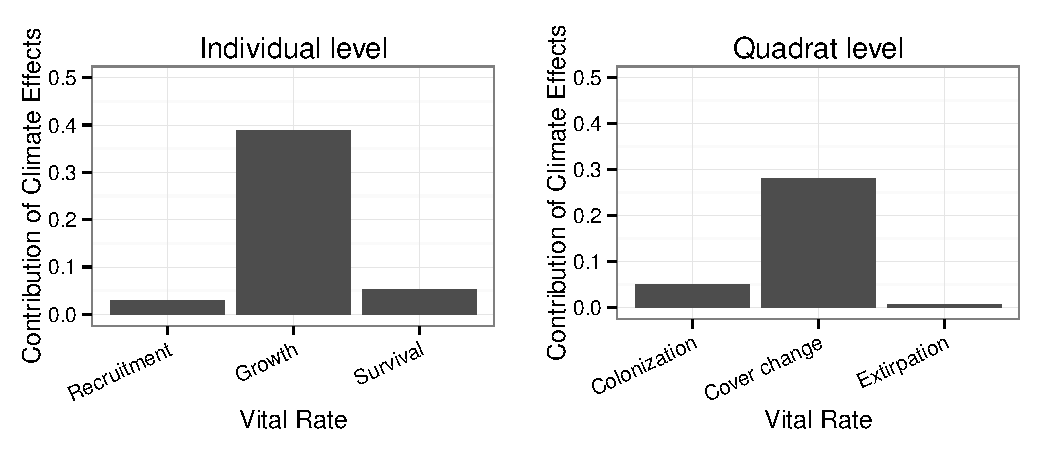
\includegraphics{components/figure/manuscript-figure_1.pdf}
\caption{Time series of average percent cover over all quadrats for our
four focal species: \emph{Bouteloua gracilis} (BOGR), \emph{Hesperostipa
comata} (HECO), \emph{Pascopyrum smithii} (PASM), and \emph{Poa secunda}
(POSE). Light grey lines show trajectories of individual quadrats. Note
the different y-axis scales across panels.}
\end{figure}

\begin{figure}[htbp]
\centering
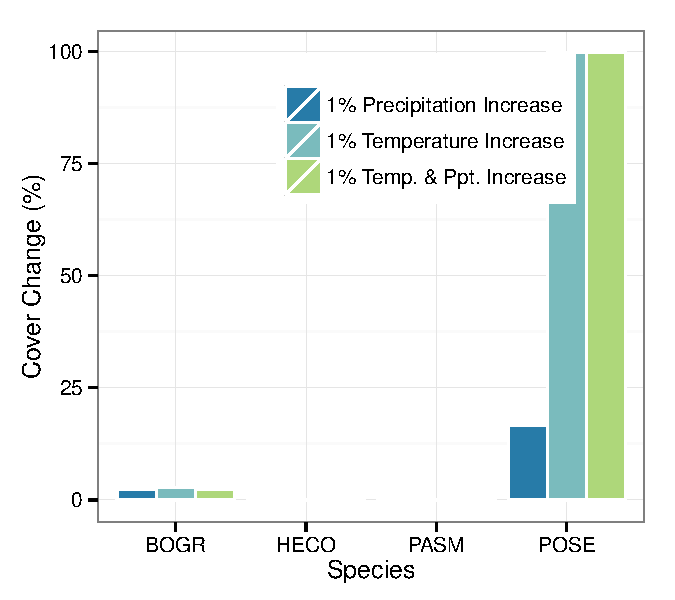
\includegraphics{components/figure/manuscript-figure_2.pdf}
\caption{Work flow of the data aggregation, model fitting, and
population simulating.}
\end{figure}

\begin{figure}[htbp]
\centering
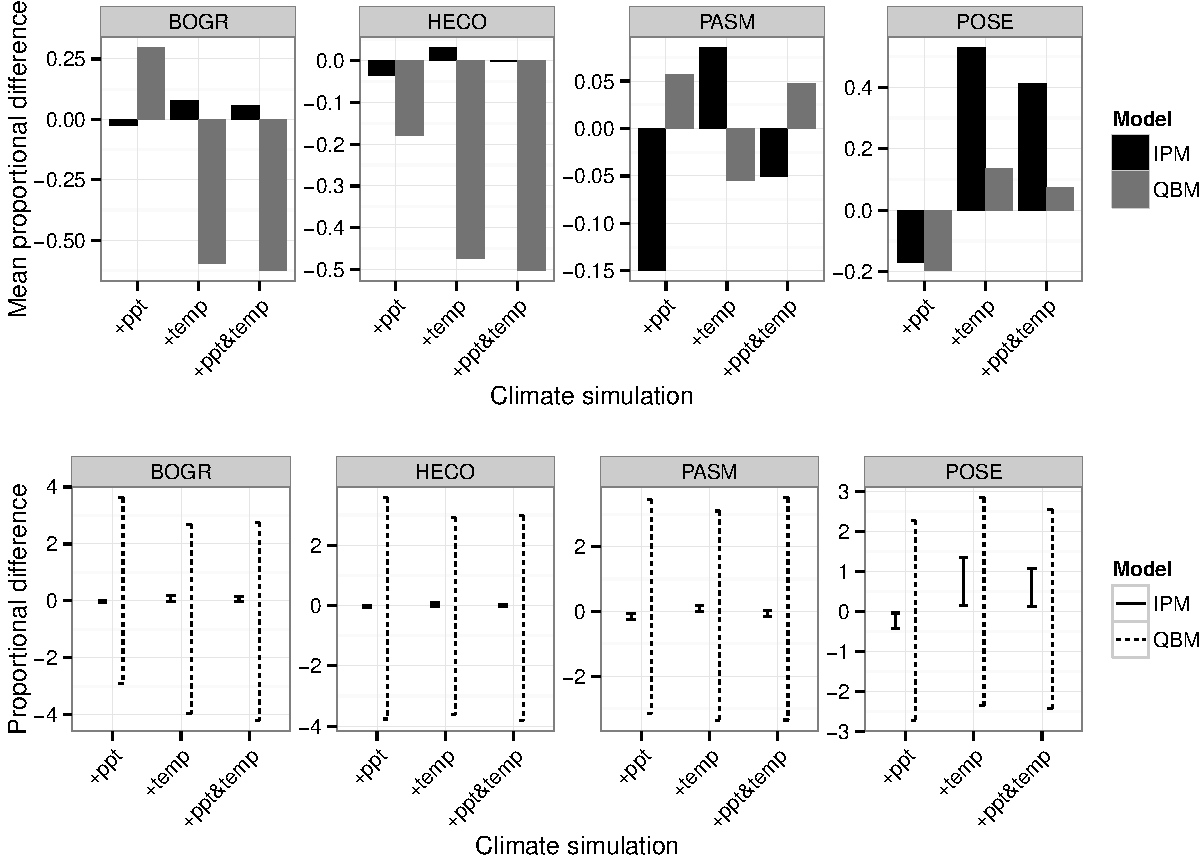
\includegraphics{components/figure/manuscript-figure_3.pdf}
\caption{Sensitivity of equilibrium cover simulated from the IPM to each
climate scenario applied to individual and combined vital rates. For
example, the points associated with G show the median cover from IPM
simulations where a climate perturbation is applied only to the growth
regression climate covariates. These simulations use mean parameter
values for clarity.}
\end{figure}

\begin{figure}[htbp]
\centering
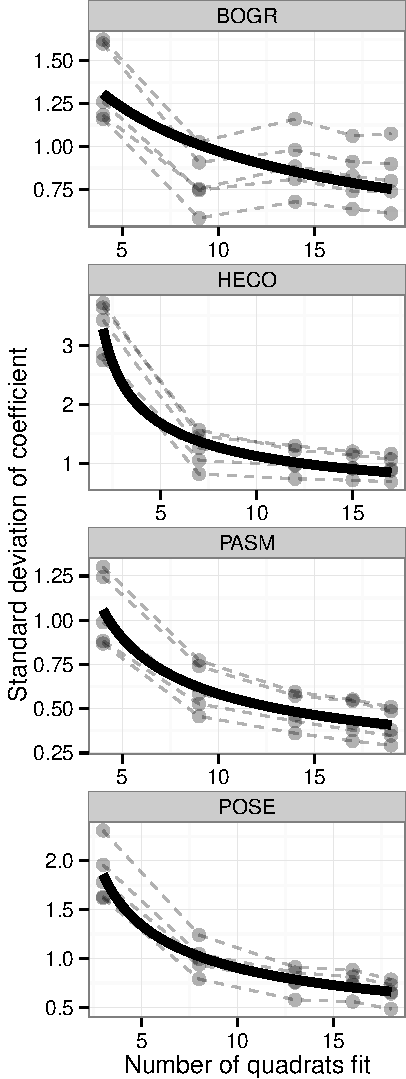
\includegraphics{components/figure/manuscript-figure_4.pdf}
\caption{Effect of quadrat sample size on the precision (standard
deviation) of main climate effect estimates in the QBM. Increasing the
number of quadrats results in diminishing returns in terms of parameter
certainty. Light dashed lines show individual climate effects at five
quadrat sample sizes. Thick dark lines are inverse gaussian fits showing
the mean effect of increasing quadrat sample size on parameter
precision.}
\end{figure}

\begin{figure}[htbp]
\centering
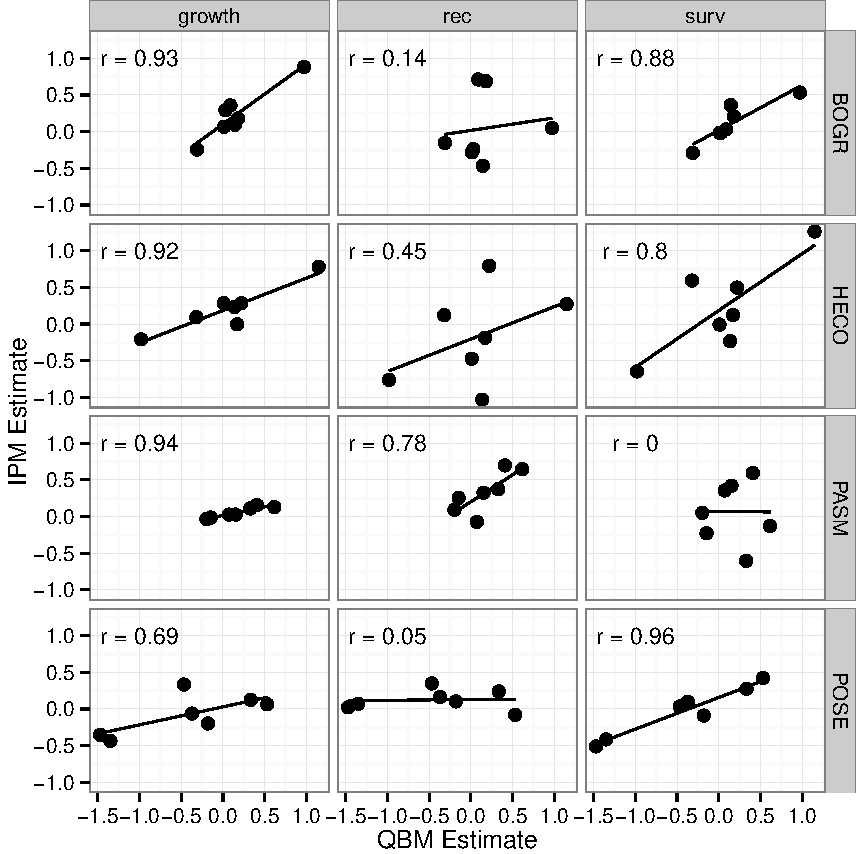
\includegraphics{components/figure/manuscript-figure_5.pdf}
\caption{Correlations (r) between QBM and IPM estimates of climate
effects. We ignore sizeXclimate interactions since these are not
directly comparable across model types. The QBM does not have multiple
vital rates, so its values are repeated across panels within each
species. Across top panels, `growth' = growth regression, `rec' =
recruitment regression, `surv' = survival regression.}
\end{figure}

\begin{figure}[htbp]
\centering
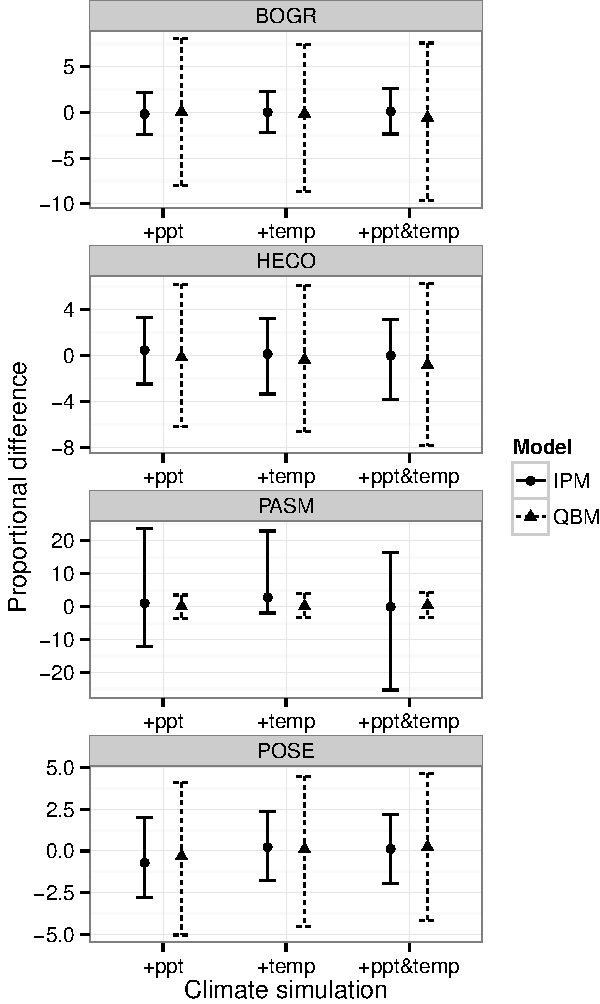
\includegraphics{components/figure/manuscript-figure_6.pdf}
\caption{Equilibrium cover and 90\% quantiles around the mean prediction
when model error and parameter uncertainty are propogated through the
simulation phase. Climate simulations are as in Figure 3.}
\end{figure}

\pagebreak{}

\subsection{References}\label{references}

Adler, P. B., H. J. Dalgleish, and S. P. Ellner. 2012. Forecasting plant
community impacts of climate variability and change: when do competitive
interactions matter? Journal of Ecology 100:478--487.

Anderson, J., L. Vermeire, and P. B. Adler. 2011. Fourteen years of
mapped, permanent quadrats in a northern mixed prairie, USA. Ecology
92:1703.

Araújo, M. B., and A. T. Peterson. 2012. Uses and misuses of bioclimatic
envelope modeling. Ecology 93:1527--1539.

Battin, J., M. W. Wiley, M. H. Ruckelshaus, R. N. Palmer, E. Korb, K. K.
Bartz, and H. Imaki. 2007. Projected impacts of climate change on salmon
habitat restoration. Proceedings of the National Academy of Sciences of
the United States of America 104:6720--6725.

Chu, C., and P. B. Adler. 2014. When should plant population models
include age structure? Journal of Ecology 102:531--543.

Chu, C., and P. B. Adler. 2015. Large niche differences emerge at the
recruitment stage to stabilize grassland coexistence. Ecological
Monographs.

Chu, C., K. M. Havstad, N. Kaplan, W. K. Lauenroth, M. P. McClaran, D.
P. Peters, L. T. Vermeire, and P. B. Adler. 2014. Life form influences
survivorship patterns for 109 herbaceous perennials from six semi-arid
ecosystems. Journal of Vegetation Science 25:947--954.

Clark, J. S., and O. N. Bjørnstad. 2004. Population time series: Process
variability, observation errors, missing values, lags, and hidden
states. Ecology 85:3140--3150.

Clark, J. S., D. M. Bell, M. H. Hersh, and L. Nichols. 2011a. Climate
change vulnerability of forest biodiversity: Climate and competition
tracking of demographic rates. Global Change Biology 17:1834--1849.

Clark, J. S., D. M. Bell, M. H. Hersh, M. C. Kwit, E. Moran, C. Salk, A.
Stine, D. Valle, and K. Zhu. 2011b. Individual-scale variation,
species-scale differences: Inference needed to understand diversity.

Clark, J. S., D. M. Bell, M. Kwit, A. Stine, B. Vierra, and K. Zhu.
2012. Individual-scale inference to anticipate climate-change
vulnerability of biodiversity. Philosophical Transactions of the Royal
Society B: Biological Sciences 367:236--246.

Clark, J. S., D. Bell, C. Chu, B. Courbaud, M. Dietze, M. Hersh, J.
HilleRisLambers, I. Ibáñez, S. LaDeau, S. McMahon, J. Metcalf, J. Mohan,
E. Moran, L. Pangle, S. Pearson, C. Salk, Z. Shen, D. Valle, and P.
Wyckoff. 2010. High-dimensional coexistence based on individual
variation: a synthesis of evidence. Ecological Monographs 80:569--608.

Clark, J. S., S. R. Carpenter, M. Barber, S. Collins, A. Dobson, J. A.
Foley, D. M. Lodge, M. Pascual, R. Pielke, W. Pizer, C. Pringle, W. V.
Reid, K. A. Rose, O. Sala, W. H. Schlesinger, D. H. Wall, and D. Wear.
2001. Ecological forecasts: an emerging imperative. Science (New York,
N.Y.) 293:657--660.

Clark, J. S., A. E. Gelfand, C. W. Woodall, and K. Zhu. 2014. More than
the sum of the parts: Forest climate response from joint species
distribution models. Ecological Applications 24:990--999.

Dalgleish, H. J., D. N. Koons, M. B. Hooten, C. A. Moffet, and P. B.
Adler. 2011. Climate influences the demography of three dominant
sagebrush steppe plants. Ecology 92:75--85.

Doak, D. F., and W. F. Morris. 2010. Demographic compensation and
tipping points in climate-induced range shifts. Nature 467:959--962.

Elith, J., and J. R. Leathwick. 2009. Species Distribution Models:
Ecological Explanation and Prediction Across Space and Time.

Freckleton, R. P., W. J. Sutherland, A. R. Watkinson, and S. A.
Queenborough. 2011. Density-structured models for plant population
dynamics. American Naturalist 177:1--17.

Galván, J. D., J. J. Camarero, and E. Gutiérrez. 2014. Seeing the trees
for the forest: Drivers of individual growth responses to climate in
Pinus uncinata mountain forests. Journal of Ecology 102:1244--1257.

Guisan, A., and W. Thuiller. 2005. Predicting species distribution:
Offering more than simple habitat models.

Hobbs, N. T., and M. B. Hooten. 2015. Bayesian Models: A Statistical
Primer for Ecologists. Princeton University PressPrinceton.

Jenouvrier, S., H. Caswell, C. Barbraud, M. Holland, J. Stroeve, and H.
Weimerskirch. 2009. Demographic models and IPCC climate projections
predict the decline of an emperor penguin population. Proceedings of the
National Academy of Sciences of the United States of America
106:1844--1847.

Lauenroth, W. K., and P. B. Adler. 2008. Demography of perennial
grassland plants: Survival, life expectancy and life span. Journal of
Ecology 96:1023--1032.

Liu, Y., Y. Jang, W. Woo, and T.-K. Kim. 2014. Video-Based Object
Recognition Using Novel Set-of-Sets Representations.

Luo, Y., K. Ogle, C. Tucker, S. Fei, C. Gao, S. LaDeau, J. S. Clark, and
D. S. Schimel. 2011. Ecological forecasting and data assimilation in a
data-rich era. Ecological Applications 21:1429--1442.

Maiorano, L., R. Cheddadi, N. E. Zimmermann, L. Pellissier, B.
Petitpierre, J. Pottier, H. Laborde, B. I. Hurdu, P. B. Pearman, A.
Psomas, J. S. Singarayer, O. Broennimann, P. Vittoz, A. Dubuis, M. E.
Edwards, H. A. Binney, and A. Guisan. 2013. Building the niche through
time: using 13,000 years of data to predict the effects of climate
change on three tree species in Europe. Global Ecology and Biogeography
22:302--317.

Pearson, R. G., and T. P. Dawson. 2003. Predicting the impacts of
climate change on the distribution of species: Are bioclimate envelope
models useful? Global Ecology and Biogeography 12:361--371.

Petchey, O. L., M. Pontarp, T. M. Massie, S. Kéfi, A. Ozgul, M.
Weilenmann, G. M. Palamara, F. Altermatt, B. Matthews, J. M. Levine, D.
Z. Childs, B. J. McGill, M. E. Schaepman, B. Schmid, P. Spaak, A. P.
Beckerman, F. Pennekamp, and I. S. Pearse. 2015. The ecological forecast
horizon, and examples of its uses and determinants. Ecology Letters
18:597--611.

Piantadosi, S., D. P. Byar, and S. B. Green. 1988. The Ecological
Fallacy. American Journal of Epidemiology 127:893--904.

Queenborough, S. A., K. M. Burnet, W. J. Sutherland, A. R. Watkinson,
and R. P. Freckleton. 2011. From meso- to macroscale population
dynamics: A new density-structured approach. Methods in Ecology and
Evolution 2:289--302.

R Core Development Team. 2013. R: A language and environment for
statistical computing.

Rees, M., and S. P. Ellner. 2009. Integral projection models for
populations in temporally varying environments. Ecological Monographs
79:575--594.

Stan Development Team. 2014a. Stan: A C++ Library for Probability and
Sampling, Version 2.5.0.

Stan Development Team. 2014b. Rstan: the R interface to Stan, Version
2.5.0.

Sæther, B. E., S. Engen, V. Grøtan, W. Fiedler, E. Matthysen, M. E.
Visser, J. Wright, A. P. Møller, F. Adriaensen, H. {Van Balen}, D.
Balmer, M. C. Mainwaring, R. H. McCleery, M. Pampus, and W. Winkel.
2007. The extended Moran effect and large-scale synchronous fluctuations
in the size of great tit and blue tit populations. Journal of Animal
Ecology 76:315--325.

Taylor, C. M., and A. Hastings. 2004. Finding optimal control strategies
for invasive species: a density-structured model for Spartina
alterniflora. Journal of Applied Ecology 41:1049--1057.

\end{document}
